% !TeX spellcheck = ru_RU
\documentclass[specialist,
substylefile = spbu_report.rtx,
subf,href,colorlinks=true, 12pt]{disser}

\usepackage{amsmath,amssymb,amsthm,amscd,amsfonts, mathtools}
\usepackage{multirow}
\usepackage{float}
\usepackage[utf8]{inputenc}
\usepackage[a4paper,
left=2cm, right=1.5cm, top=2cm, bottom=2cm]{geometry}
\usepackage{graphicx}
\usepackage[russian]{babel}
\usepackage{xcolor}
\usepackage{float}

\makeatletter
\newcommand*{\rom}[1]{\expandafter\@slowromancap\romannumeral #1@}
\newcommand\setItemnumber[1]{\setcounter{enum\romannumeral\@enumdepth}{\numexpr#1-1\relax}}
\makeatother


\setcounter{tocdepth}{3}
\setcounter{secnumdepth}{3}


\newtheorem{defenition}{Определение}
\newtheorem*{purpose*}{Цель работы}
\newtheorem*{prob_task*}{Вероятностная постановка задачи классификации}
\newtheorem*{algo_task*}{Алгоритмическая постановка задачи классификации}
\newtheorem*{prob_def*}{Вероятностное определение $w_{ij}^k$}
\newtheorem*{algo_def*}{Алгоритмическое определение $w_{ij}^k$}

\begin{document}
	\institution{%
		Санкт-Петербургский государственный университет\\
		Прикладная математика и информатика
	}
	
	\title{Отчет по Научно-исследовательской работе}	
	\topic{Задачи классификации мозговой активности при помощи синолитических сетей}	
	\author{Власенко Даниил Владимирович}
	\group{группа 19.Б04-мм}
	\sa{Шпилёв Пётр Валерьевич\\
		Кафедра Статистического Моделирования}
	\sastatus {к.\,ф.-м.\,н., доцент}	
	\city{Санкт-Петербург}
	\date{\number\year}	
	\maketitle
	\tableofcontents
	
	\intro
		\section{Функциональная магнитно-резонансная томография}
			Функциональная магнитно-резонансная томография или фМРТ — разновидность магнитно-резонансной томографии, которая проводится с целью измерения изменений в токе крови, вызванных нейронной активностью головного мозга. 
			
			Этот метод основывается на том, что мозговой кровоток и активность нейронов связаны между собой. Когда область мозга активна, приток крови к этой области также увеличивается. 
			
			Испытуемый помещается в фМРТ аппарат, снимки мозга испытуемого происходят последовательно с интервалом в несколько секунд или миллисекунд. Таким образом результатом работы фМРТ аппарата является объемное трехмерное изображение, изменяющееся во времени, в центре которого расположен зафиксированный неподвижный мозг. Значение вокселя фМРТ в конкретный момент времени отображает концентрацию крови в данной области мозга.
	
			фМРТ позволяет определить активацию определенной области головного мозга во время нормального его функционирования под влиянием различных факторов (например, движение тела) и при различных патологических состояниях. Эти знания помогают понять, как из согласованной работы частей мозга складываются высшие психические функции, такие как память, внимание, мышление. 
			
			На сегодняшний день это один из самых активно развивающихся видов нейровизуализации. С начала 1990-х годов фМРТ стала доминировать в области визуализации процессов головного мозга из-за своей сравнительно низкой инвазивности, отсутствия воздействия радиации и относительно широкой доступности.
			
			Большой интерес вызывает способность различать поведение человека и его деятельность на основе данных нейровизуализации. Будем считать, что мозг может функционировать в двух режимах. Как по результатам фМРТ сканирования определить, в каком из двух режимов был мозг? 
			
		\section{Векторизация данных фМРТ}
			Результатом работы фМРТ сканера является последовательность трехмерных изображений, таким образом \ Omagaницей данных является воксель изображения в конкретный момент дискретного времени. Наиболее распространенным форматом хранения фМРТ данных является NIFTI формат. Библиотека Nibabel~\cite{BrettMatthew2023} позволяет читать NIFTI формат и представляет его в памяти как четырехмерный массив положительных действительных чисел, где первые три индекса фиксируют положение вокселя в пространстве, а четвертый отвечает за время. Значения массива отображают концентрацию крови в данном вокселе в данный момент времени.
			
		\section{Представление мозга как сети}
			Мозг --- это сложная сеть, а фМРТ отражает работу этой сети во времени. Для эффективной классификации на основе такого сложного типа больших данных нужно использовать методы, которые будут учитывать взаимосвязи между элементами входящими в сеть.
			
			Идея данной работы заключается в том, чтобы строить на основе данных фМРТ графы, вершины которых будут отражать области мозга, а веса ребер – взаимосвязь между областями при конкретном режиме мозговой активности. После подобного представления мозга будут использоваться методы машинного обучения, которые будут учитывать характеристики графов при обучении модели и последующей классификации.
			
			\begin{figure}[h]
				\centering
				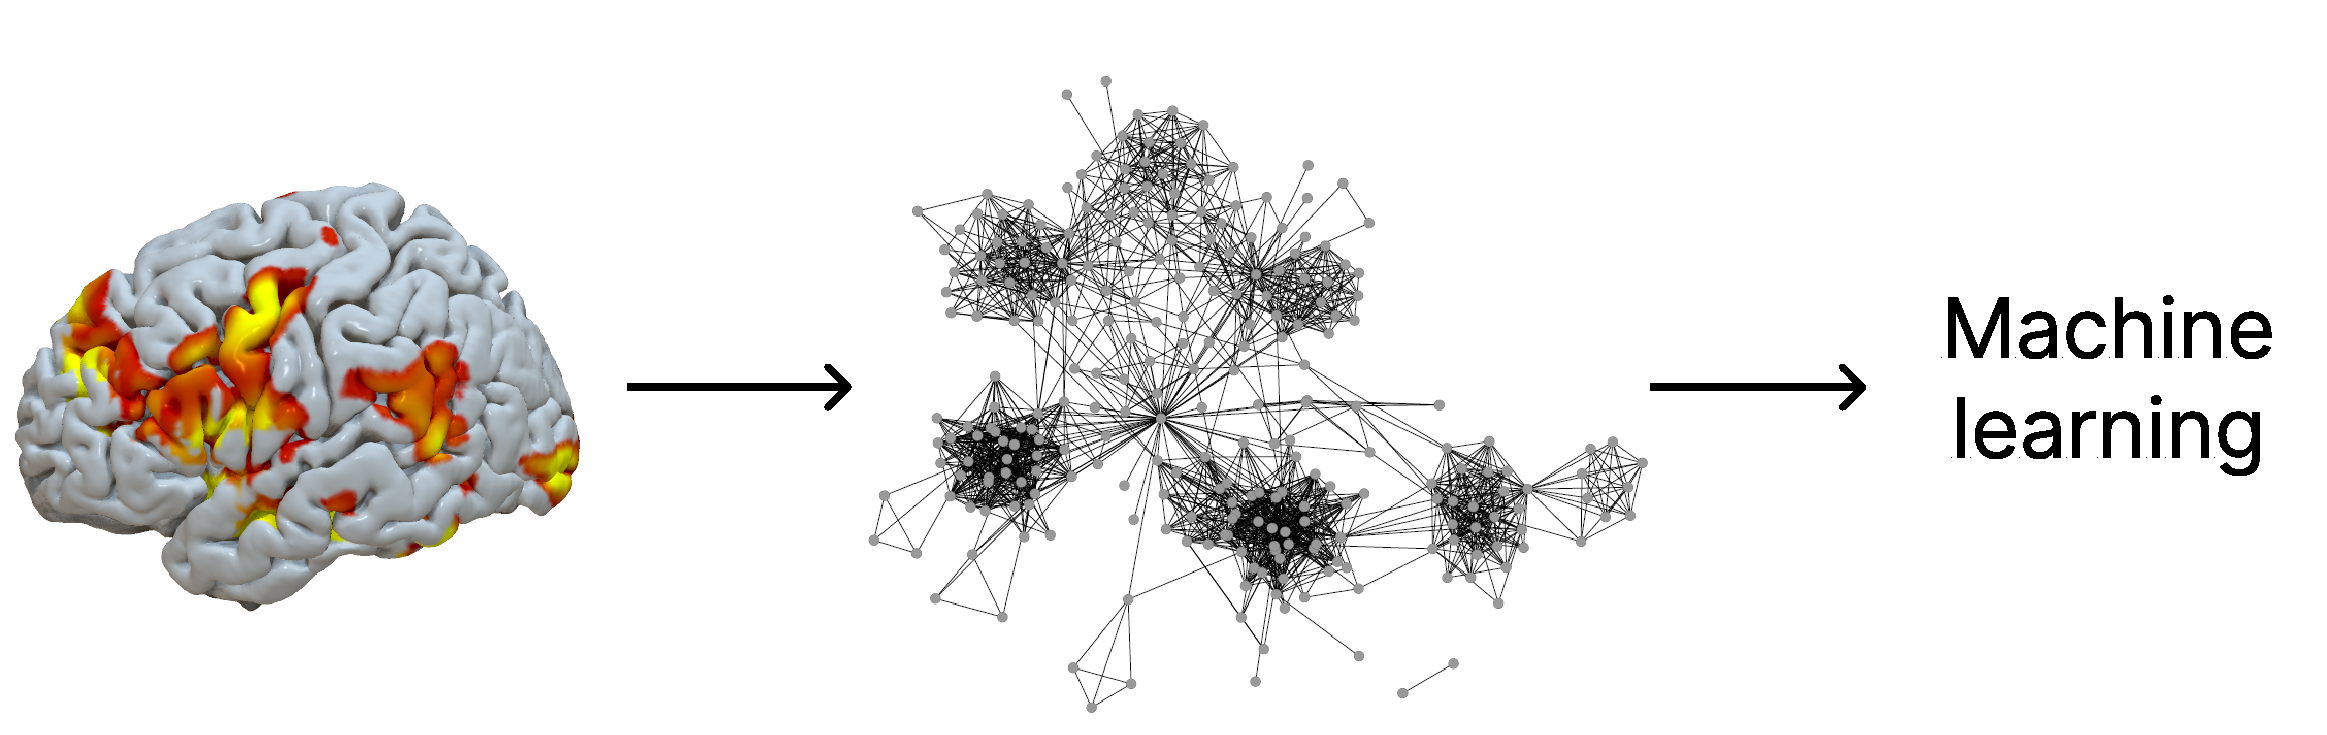
\includegraphics[width=12cm]{../images/fmri_graph_ml_1.pdf}
				\caption{Идея работы.} 
				\label{fg:1}
			\end{figure}
			
			Метод построения графов, который я модифицировал для поставленной задачи и который изложу далее, называется синолитическим. Его эффективность при классификации была подтверждена при исследованиях других типов биологических данных~\cite{DemichevV2022, Krivonosov2020}.						
		
			\begin{purpose*}
				Реализация и тестирование метода классификации режимов мозговой активности на основе фМРТ данных, в основе которого будут лежать синолитические сети.
			\end{purpose*}				
		
	\chapter{Модель}	
		\section{Классификация}
		Для дальнейшей работы формализуем термин “классификация”. 
		\begin{defenition}
			Пусть $\Omega$ --- множество объектов, $\Sigma$ --- множество классов. Существует неизвестная функция $f: \Omega \rightarrow \Sigma$, значения которой известны только на объектах выборки $(\widetilde{\Omega}, \widetilde{\Sigma}) =  \{(\omega_{n}, \sigma_{n})\}_n$. Требуется построить алгоритм $\widehat{f}: \Omega \rightarrow \Sigma$, способный классифицировать произвольный объект $\omega \in \Omega$, то есть правильно сопоставить ему соответствующий класс $\sigma \in \Sigma$.
		\end{defenition}
		
		Такой алгоритм $\widehat{f}$ будем называть моделью. Таким образом требуется построить модель $\widehat{f}$, которая смогла бы по данным фМРТ определить в каком из двух режимов мозговой активности был мозг при сканировании.								
		
		\section{Построение графа на основе фМРТ}
			Метод построения графов, модифицированный под задачи классификации мозговой активности на основе фМРТ данных и изложенный в этом разделе, называется синолитическим. Каждая вершина в графе будет отражать воксель в фМРТ данных, ребра между вершинами и веса ребер будут отражать взаимосвязь вокселей. 		
			
			Множество фМРТ будем обозначать $\Omega$, а множество режимом мозговой активности~--- $\Sigma = \{$\rom{1}, \rom{2}$\}$. $(\widetilde{\Omega}, \widetilde{\Sigma}) =  \{(\omega_{n}, \sigma_{n})\}_n$ --- конечная выборка из $(\Omega, \Sigma)$, необходимая для построения и обучения модели.	
			
			Сначала с помощью библиотеки Nibabel $\omega \in \Omega$ конвертируется в четырехмерный массив~$a$. Первые три индекса $x$, $y$, $z$ фиксируют положение вокселя фМРТ, а четвертый индекс $t$ отвечает за время. Таким образом через $a_{xyzt}$ будем обозначать значение вокселя с индексами $x$, $y$, $z$ в момент времени $t$, а через $a_{xyz}$ будем обозначать все значения вокселя с индексами $x$, $y$, $z$. Иногда будет
			удобно использовать для индексации конкретного вокселя не три целых числа, а одно. Для этого положим, что все воксели в пространстве проиндексированы натуральными числами.	
			
			На основе массив $a$ в дальнейшем будет строится граф $g = (V, E, R, W)$, где $V = \{v_i\}_i$~--- множество вершин, $E = \{e_{ij}\}_{ij}$~--- множество неориентированных ребер, $R = \{r_i\}_i$~--- множество значений вершин, $W = \{w_{ij}\}_{ij}$~--- множество весов ребер, $v_i$~--- вершина, отражающая воксель $i$, $e_{ij}$~--- ребро, отражающее связь между вокселями $i$ и $j$, $r_i$~--- значение вершины $v_i$, $w_{ij}$~--- вес ребра $e_{ij}$.
			
			Обсудим как вычисляются значения вершин $R$. Как было сказано выше вершина $v_i$ отражает собой воксель $i$ и у нее есть значение $r_i$, но воксель $i$ это временной ряд с множеством значений. Для вычисления $r_i$ в модели используется статистика $T$, которая будет преобразовывать все значения вокселя в одно число. Таким образом можно ввести новый трехмерный массив $a^{T} = T(a)$, т.е для $\forall x, y, z$ $a^{T}_{xyz} = T(a_{xyz})$. Значения массива $a^{T}$ и будут использоваться в качестве значений вершин $R$. Статистика $T$ будет выбираться исходя из результатов тестирования модели.
			
			Наиболее важно то, каким образом вычисляются значения весов ребер $W$, потому что веса ребер отражают взаимосвязь между вокселями при разных режимах работы мозга. Дадим сначала теоретическое определение для $w_{ij}$:					
			\begin{equation}
				w_{ij} = P(\sigma = \rom{2} | r_i, r_j) - P(\sigma = \rom{1} | r_i, r_j)
				\label{eq:1}
			\end{equation}		
			Таким образом вес ребра $w_{ij}$ равен разнице вероятностей режимов работы мозга при условии значений инцидентных ребру вершин и принимает значения от $-1$ до $1$. Соответственно, если вес ребра $w_{ij} < 0$ , то ребро $e_{ij}$ несет в себе информацию о том, что более вероятно, что фМРТ было сканировано с мозга, который находился в режиме \rom{1}, а если вес ребра $w_{ij} > 0$, то данное ребро несет в себе информацию о том, что более вероятно, что фМРТ было сканировано с мозга, который находился в режиме \rom{2}. Чем больше вес ребра $|w_{ij}|$ тем больше информации для классификации несет в себе ребро $e_{ij}$.
		
			На практике для вычисления таких вероятностей используются вероятностные классификаторы $Cl_{ij}: \{\sigma |(r_i, r_j), \{(r_i^n, r_j^n)\}_n, \{\sigma_n\}_n\} \rightarrow [0, 1]$, которые обучаются на имеющейся выборке $(\widetilde{\Omega}, \widetilde{\Sigma})$. Можно переписать формулу~\eqref{eq:1} так:
			\begin{equation}
				\begin{multlined}
					w_{ij} = Cl_{ij}(\sigma = \rom{2} | (r_i, r_j), \{(r_i^n, r_j^n)\}_n, \{\sigma_n\}_n) - \\ - Cl_{ij}(\sigma = \rom{1} | (r_i, r_j), \{(r_i^n, r_j^n)\}_n, \{\sigma_n\}_n)
				\end{multlined}
				\label{eq:2}
			\end{equation}
			Таким образом для каждого ребра $e_{ij}$ требуется обучить свой вероятностный классификатор $Cl_{ij}$ для последующего вычисления весов ребер $W$. В данной работе используются вероятностные классификаторы $Cl_{ij}$, в основе которых лежит метод опорных векторов с радиально-базисным ядром~\cite{Platt1999}.
			
			Теперь когда известно каким образом считаются значения вершин $R$ и значения весов ребер $W$, можно описать топологию графа. Как правило при построении синолитических сетей строится полный граф, что позволяет учитывать взаимодействия между всеми элементами сети. В случае данных фМРТ вершин в графе получается много, что приведет такому количеству ребер при построении полного графа, что модель будет неэффективной. Например, если разрешение фМРТ $100\times100\times100$ вокселей, то в графе будет $1.000.000$ вершин и $\frac{1.000.000 \cdot 999.999}{2} = 499.999.500.000$ ребер. И для каждого ребра $e_{ij}$ нужно обучать свой классификатор $Cl_{ij}$, это приводит к большим затратам памяти и вычислительного времени.
			
			Вместо полного графа предлагается строить а граф-сетку, то есть такой граф, в котором каждый внутренний воксель связан с 26 своими соседями. То есть воксель $(xyz)$ связан с вокселями из множества $\{(\hat{x}\hat{y}\hat{z}): \hat{x} \in \{x- 1,x, x +1\}, \hat{y} \in \{y- 1,y, y +1\}, \hat{z} \in \{z- 1,z, z +1\}, (\hat{x}\hat{y}\hat{z}) \neq (xyz)\}$. При такой топологии графа затраты на память и вычислительное время сократятся с $O(n^2)$ до $O(n)$.
			
			Так как в фМРТ изображен не только мозг, но и пространство вокруг головы испытуемого, следует удалить из графа ребра, которые инциденты с вершинами, значения которых ниже порогового значения $r$. Такие ребра не несут полезной информации для классификации. Так же из графа следует удалить ребра, абсолютное значение веса которых ниже порогового значения $w$. Ребра, абсолютное значение веса которых близко к нулю, так же не несут полезной информации для классификации.
			
		\section{Классификация на основе характеристик графа}
			После построения графа $g$ вычисляются его характеристики $\{f_u\}_u = \{F_u(g)\}_u$, таким образом от графа остается последовательность чисел $\{f_u\}_u$. В качестве характеристик графа $\{F_u(g)\}_u$ могут выступать среднее весов ребер, дисперсия весов ребер, количество компонент связности и т.д. Характеристики $\{F_u(g)\}_u$ выбираются по результатам работы модели. На основе $\{f_u\}_u$ происходит итоговая классификация фМРТ данных $\omega$ с помощью классификатора $Cl$, который был обучен на выборке $\{\{f_u^n\}_u\}_n$. В качестве классификатора в работе использовался классификатор, основанный на методе опорных векторов с радиально-базисным ядром.
			
		\section{Алгоритм}
			Изложим теперь алгоритмы обучения модели и классификации с ее помощью. 
						
			\subsection{Обучение}
				Входные данные: выборка $(\widetilde{\Omega}, \widetilde{\Sigma})$, статистика вокселей $T$, минимальное значение вершины $r$, для которого инцидентные с ним ребра не удаляются из графа, минимальное абсолютное значение ребра $w$, для которого ребро не удаляется из графа, характеристики графов $\{F_u\}_u$, на которых будет обучаться модель.			
				
				Последовательность шагов обучения модели:
				\begin{enumerate}
					\item Построение $\{a^n\}_n$ для $\forall \omega \in \widetilde{\Omega}$;
					\item Вычисление $\{a^{Tn}\}_n$ и, соответственно, $R$ с помощью $T$;
					\item Обучение  $\{Cl_{ij}\}_{ij}$ на выборке $(\{(r_i^n, r_j^n)\}_n, \{\sigma_n\}_n)$ для $\forall e_{ij} \in E$;
					\item Вычисление $\{W_n\}_n = \{\{w_{ij}^n\}_{ij}\}_n$ с помощью $\{Cl_{ij}\}_{ij}$ и $R$;
					\item Построение графов-сеток $\{g_n\}_n$;
					\item Удаление ребер $\{e_{ij}^n : r_i^n < r | r_j^n < r | w_{ij}^n < w\}_{ij}$  для $\forall g_n$;
					\item Вычисление $\{\{f^n_u\}_u\}_n = \{\{F_u(g_n)\}_u\}_n$;
					\item Обучение $Cl$ на выборке $\{\{f^n_u\}_u\}_n$.
				\end{enumerate}
			
			\subsection{Классификация}
				Входные данные: фМРТ $\omega$, статистика вокселей $T$, минимальное значение вершины $r$, для которого инцидентные с ним ребра не удаляются из графа, минимальное абсолютное значение ребра $w$, для которого ребро не удаляется из графа, характеристики графов $\{F_u\}_u$, на которых будет обучаться модель.
				
				Последовательность шагов классификации с помощью модели:				
				\begin{enumerate}
					\item Построение $a$;
					\item Вычисление $a^{T}$ и, соответственно, $R$ с помощью $T$;
					\item Вычисление $W = \{w_{ij}\}_{ij}$ с помощью $\{Cl_{ij}\}_{ij}$ и $R$;
					\item Построение графа-сетки $g$;
					\item Удаление ребер $\{e_{ij} : r_i < r | r_j < r | w_{ij} < w\}_{ij}$  для $g$;
					\item Вычисление $\{f^n_u\}_u = \{F_u(g)\}_u$;
					\item Классификация $\{f^n_u\}_u$ с помощью $Cl$.
				\end{enumerate}

	\chapter{Тестирование модели}	
		В данной главе изложена информация о данных, на которых тестировалась модель, информация о характеристиках полученных графов и результаты модели.
		
		\section{Данные}	
			Модель была протестирована на следующих данных~\cite{Horikawa2019}, рисунок~\ref{fg:2}. Есть два режима, в которых может функционировать мозг испытуемого. Первый режим – испытуемому последовательно показывают 55 блоков, 50 из которых различные между собой изображения, 5 – повторяют предшествующую картинку. Если испытуемый видит повторную картинку, он должен нажать на кнопку. Это нужно для поддержания внимания испытуемого. Второй режим – испытуемого последовательно просят представить 25 объектов. После представления каждого объекта испытуемого просят оценить по пятибалльной шкале степень ясности образа, который он представил, с помощью нажатия кнопок.
			
			\begin{figure}[h]
				\centering
				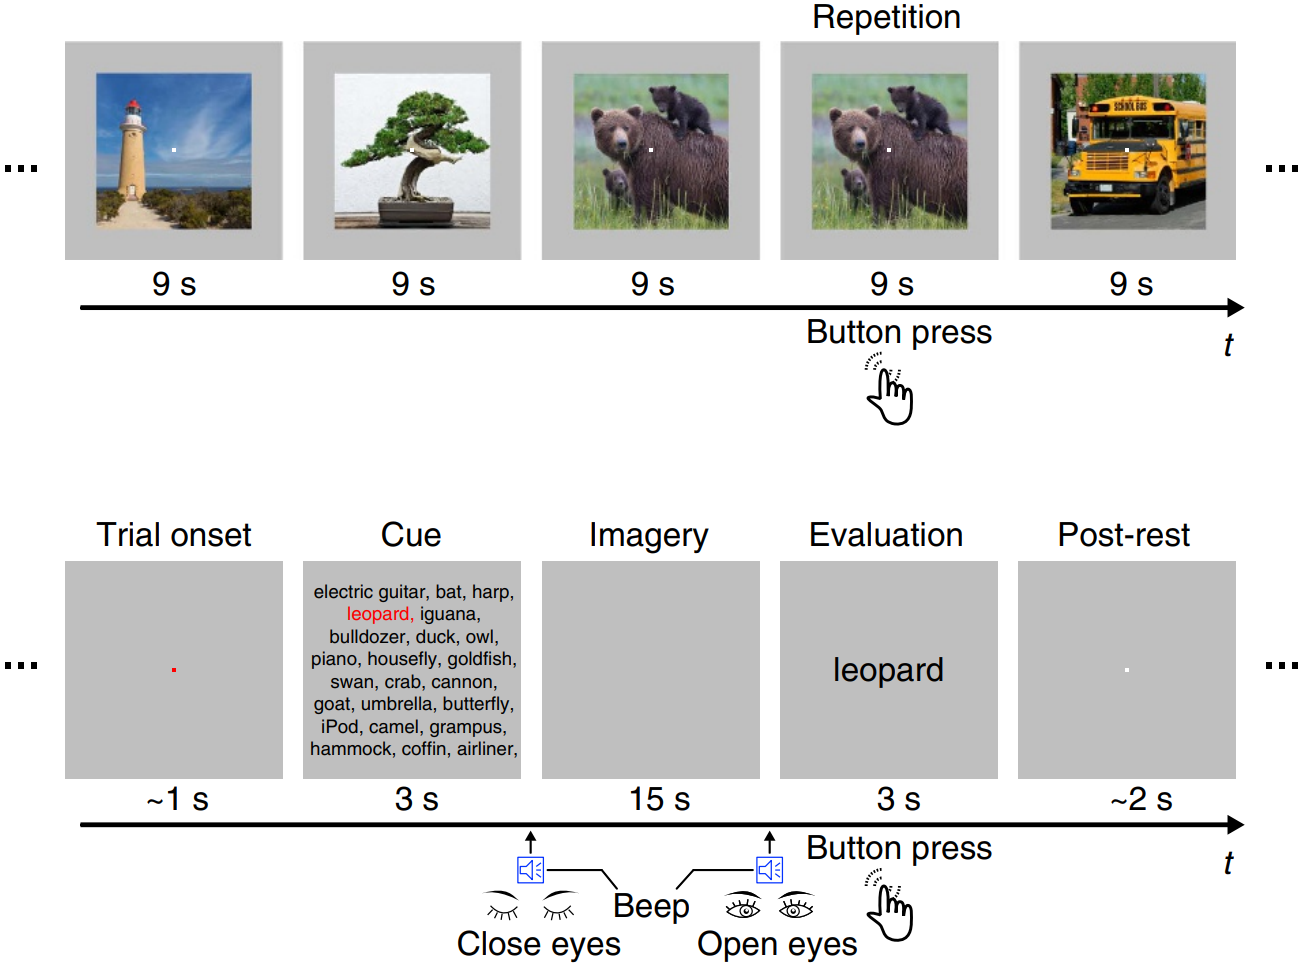
\includegraphics[width=12cm]{../images/data_3.png}
				\caption{Наблюдение или воображение объекта.} 
				\label{fg:2}
			\end{figure}
		
			В сборе данных участвовало 5 испытуемых, у каждого было сканировано в разные дни 44 фМРТ в двух режимах, из которых 24 в режиме зрительного восприятия и 20 в режиме визуализации на основе памяти. Выборка была разделена таким образом, что 30\% выборки каждого режима попадает в тестовую выборку и 70\% в обучающую. В таблице~\ref{tb:1} представлена информация о выборке фМРТ и о ее разделение на тестовую и обучающую части. 
			
			\begin{table}[h]
				\centering
				\begin{tabular}{c|cc|cc|c}
					& \multicolumn{2}{c|}{seen}            & \multicolumn{2}{c|}{imagined}        &                      \\ \cline{2-5}
					& \multicolumn{1}{c|}{training} & test & \multicolumn{1}{c|}{training} & test &                      \\ \hline
					sub-01 & \multicolumn{1}{c|}{17}       & 7    & \multicolumn{1}{c|}{14}       & 6    & 44                   \\
					sub-02 & \multicolumn{1}{c|}{17}       & 7    & \multicolumn{1}{c|}{14}       & 6    & 44                   \\
					sub-03 & \multicolumn{1}{c|}{17}       & 7    & \multicolumn{1}{c|}{14}       & 6    & 44                   \\
					sub-04 & \multicolumn{1}{c|}{17}       & 7    & \multicolumn{1}{c|}{14}       & 6    & 44                   \\
					sub-05 & \multicolumn{1}{c|}{16}       & 8    & \multicolumn{1}{c|}{14}       & 6    & 44                   \\ \hline
					& \multicolumn{1}{c|}{84}       & 36   & \multicolumn{1}{c|}{70}       & 30   & \multirow{2}{*}{220} \\ \cline{2-5}
					& \multicolumn{2}{c|}{120}             & \multicolumn{2}{c|}{100}             &                     		
				\end{tabular}				
				\caption{\label{tb:1}Разделение выборки.} 
			\end{table}
		
			Оригинальное разрешение фМРТ данных в было $3 \times 3 \times 3$ мм, для уменьшения затрат вычислительных ресурсов и сглаживания индивидуальных особенностей строения мозга качество фМРТ данных было понижено до $10 \times 10 \times 10$ мм.
	
		\section{Распределения характеристик графов}
			На графиках \ref{fg:3} и \ref{fg:4} представлена информация о распределениях трех характеристик графов, а именно о среднем весов ребер, квантиле уровня $0.9$ весов ребер и дисперсии весов ребер, когда $T$ --- среднее значение вокселя.
			
			Можно заменить, что объекты довольно явно разделяются визуально на две группы по классу. Эти характеристики лучше всего себя показали при классификации.
		
			\begin{figure}[h]
				\centering
				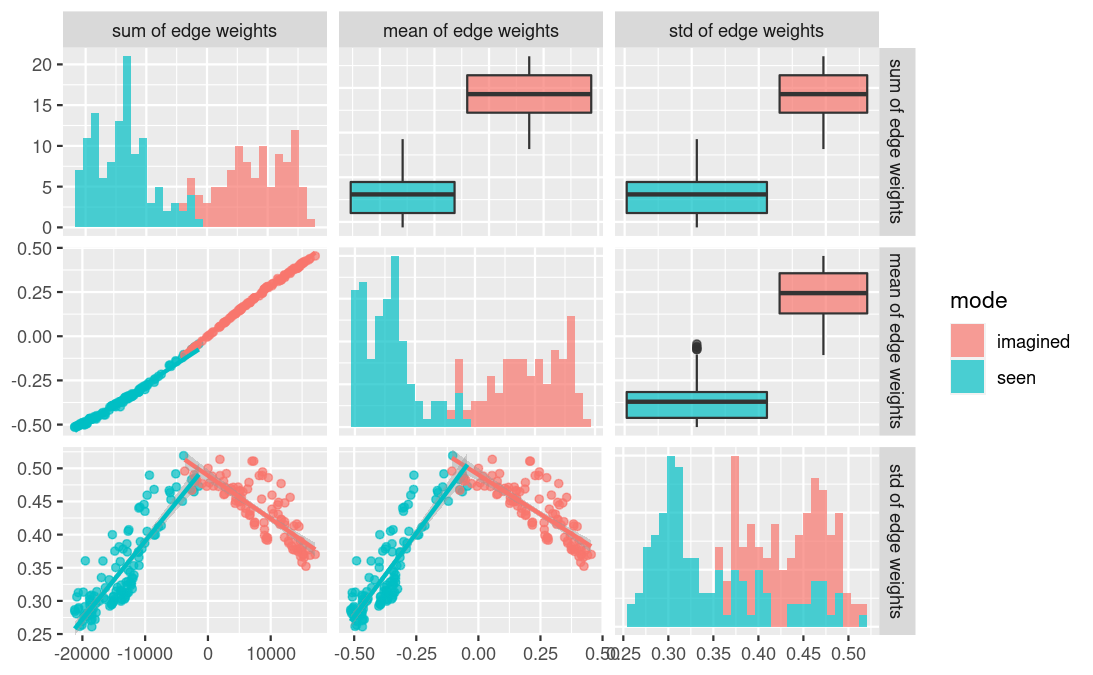
\includegraphics[width=15cm]{../images/graph_feachers_1.png}
				\caption{Распределения некоторых характеристик графов при.} 
				\label{fg:3}
			\end{figure}
		
			\begin{figure}[t!]
				\centering
				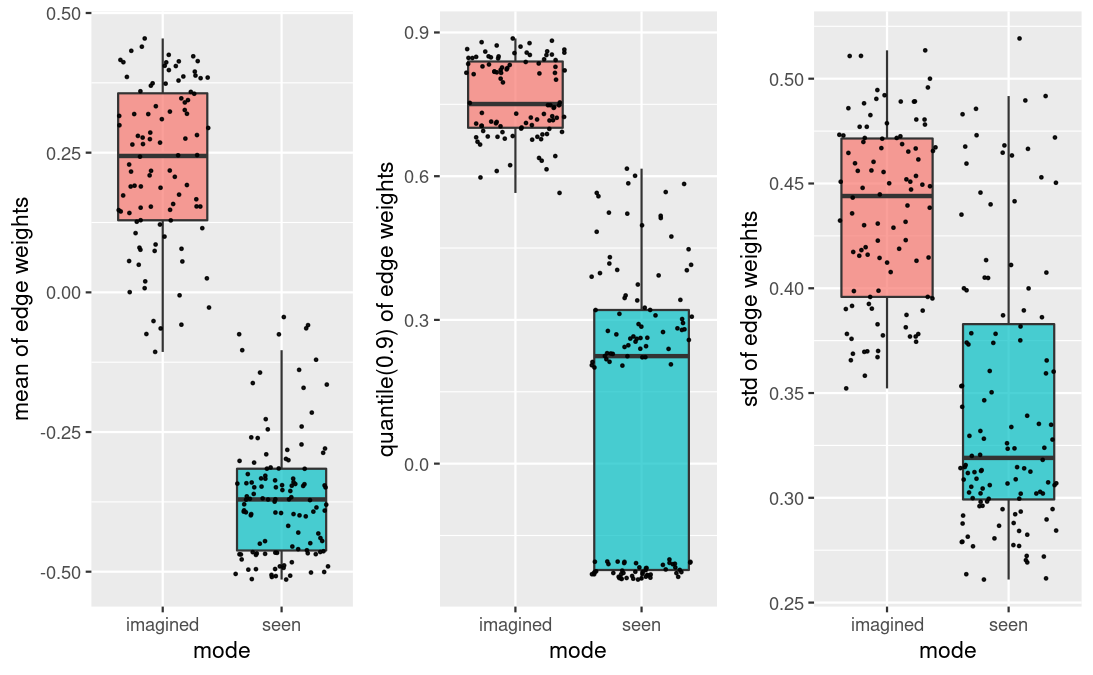
\includegraphics[width=15cm]{../images/graph_feachers_2.png}
				\caption{Распределения некоторых характеристик графов при.} 
				\label{fg:4}
			\end{figure}						 
		
		\section{Результаты классификации}
			В таблицах классификаций \ref{tb:2}, \ref{tb:3} и \ref{tb:4} представлены некоторые результаты классификации для разных статистик $T$. Лучшая точность была получена, когда $T$ --- разница квантилей уровня $0.9$ и $0.1$ вокселя, а именно $95.5\%$.
						
			\begin{table}[H]				
				\centering			
				\begin{tabular}{c|cc}
					& \multicolumn{1}{c|}{seen} & imagined \\ \hline
					seen     & 32                        & 4        \\ \cline{1-1}
					imagined & 0                         & 30      
				\end{tabular}
				\caption{\label{tb:2}$T$ --- среднее вокселя, точность $93.9\%$.}
			\end{table}			
			{
			\begin{table}[H]
				\centering				
				\begin{tabular}{c|cc}
					& \multicolumn{1}{c|}{seen} & imagined \\ \hline
					seen     & 32                        & 4        \\ \cline{1-1}
					imagined & 1                         & 29      
				\end{tabular}
				\caption{\label{tb:3}$T$ --- минимум вокселя, точность $90.9\%$.}
			\end{table}
			
			\begin{table}[H]
				\centering
				\begin{tabular}{c|cc}
					& \multicolumn{1}{c|}{seen} & imagined \\ \hline
					seen     & 34                        & 2        \\ \cline{1-1}
					imagined & 1                         & 29      
				\end{tabular}
				\caption{\label{tb:4}$T$ --- разница квантилей уровня $0.9$ и $0.1$ вокселя, точность $95.5\%$.}
			\end{table}
			}
	\conclusion
		Была изучена тема синолитических сетей и их применения к анализу сложных больших данных. Был модифицирован и реализован метод классификации на основе синолитических сетей для режимов мозговой активности по данным фМРТ. В итоге, была доказана эффективность синолитических сетей в анализе и обработке мозговой активности. С исходным кодом работы можно ознакомиться на GitHub~\cite{Vlasenko2023}.
	   
	\bibliographystyle{ugost2008mod}
	\bibliography{references}
	
	
	
\end{document}
